\documentclass{article}
\usepackage{graphicx} % Required for inserting images
\usepackage{amsmath}
\usepackage[english, russian] {babel}
\usepackage[utf8]{inputenc}
\usepackage[T2A]{fontenc}
\usepackage{minted}
\usepackage{float}
\usepackage{amssymb}
\usepackage{mathtools}

\title{Компьютерная графика}
\author{Harpie}
\date{February 2025}

\begin{document}

\maketitle

\textbf{17.02.25}

\section{Собъективно-ориентированное программирование}

Это парадигма программирования которая представляет отрезок вменении во время которого возникают определенные события. Программа выполняется не линейно, программа описывается как набор обработчиков/ обработчик события.

Некоторые события происходят автоматически, какие то нужно/можно инициализировать.

Примеры обработчиков:

Paint

Load

Resize

\vspace{5mm}

Некоторые обработчики могут быть инициализированы

Refresh

\section{Полигональная КГ}

Объект описывается с помощью вершин/точек, которые соединенны отрезками. Перед описанием объекта нужно знать и задать координаты точек.

\section{Модели}

Модель строиться набором отрезков, которые определенным образом соединенны в точках, в некоторой системе координат. \textbf{Модельная система координат, объектная система координат,локальная система координат}

Правая система координат - система повернута против часовой стрелки под 90 градусов

Система координат экрана - (нужно заполнить тут) 

Правая декартовая СК (мировая система координат) - "виртуальный мир", в котором существеют модели.

\section{Кадрирование}

Операция кадрирования - совмещенние одного кадра с другим, преобразования одного кадра

Кадр - прямоуглник, стороны которого парарлельны осям координат и у которого есть параметры
 
Размер по горизонтале - Vx

Размер по вертикале - Vy

Координты нижного угла -  Vcx, Vcy


Исходный кадр обозоначается как - Wx, Wy, Wcx, Wcy

Безразмерные координаты :


$x_1 = x-V_cx$ \hspace{21mm} $y_1 = y-V_cy$
\vspace{1mm}

$x_2 = \frac{x-V_cx}{V_x}$ \hspace{22mm} $y_2 = \frac{y-V_cy}{V_y}$
\vspace{1mm}

$x_3 = \frac{x-V_cx}{V_x}*W_x$ \hspace{15mm} $y_3 = \frac{y-V_cy}{V_y}*W_y$
\vspace{1mm}

$x' = \frac{x-V_cx}{V_x}*W_x+W_cx$ \hspace{3mm} $y' = \frac{y-V_cy}{V_y}*W_y+W_cy$

\vspace{5mm}


Если умножить на - 1 еденицу, то картинка перевернется (касается перевернутых картинок)

$x_4=\frac{x-V_cx}{V_x}*W_x+W_cx$ \hspace{3mm}  $y_4= \frac{y-V_cy}{V_y}*W_y-W_cy$

\vspace{1mm}

$x_5 = \frac{x-V_cx}{V_x}*W_x+W_cx$ \hspace{3mm} $y_5 = \frac{y-V_cy}{V_y}*W_x+2W_cy$


$x' = \frac{x-C_cx}{V_x}* W_x+W_cx$ \hspace{3mm}$y' = W_cy- \frac{x-C_cx}{V_x}* W_y$

\vspace{5mm}

\textbf{24.02.25}

\textbf{Продолжение}

$x' = \frac{x-V_{cx}}{V_x} * W_x+W_c$

\vspace{5mm}

$y' = W_y - \frac{y-V_{cy}}{V_y} * W_y$


\section{Преобразование изображения}
\subsection{Элементарные преобразования}

\textbf{1. Перенос/Сдвиг}

Смысл преобразования: объект в одной системе координат 
нужно сдвинуть в "другую систнму координат".

Пример: 

$x_1 \implies x'_1$ между ними расстояние $T_x$ \hspace{5mm} $y_1 \implies y'_1$ между ними расстояние $T_y$

$x_2 \implies x'_2$ между ними расстояние $V_x$ \hspace{5mm} $y_2 \implies y'_2$ между ними расстояние $V_y$


Итог: $x'=x+T_x$ \hspace{5mm} $y'=y+T_y$

\vspace{5mm}

\textbf{2. Масштабирвоание относительно начала координат}

Это озночает, все точки преобразуются за исключением начальной точки.
На месте остается только точка начала координат.

Пример:

$3 \implies 4.5$ и т.д

Итог: $x'=x*S_x$ \hspace{5mm} $y'=y*S_y$ 

\vspace{5mm}

\textbf{3. Поворот относительно начала координат против часовой стрелки на угол $\vartheta$}

Нужно соеденить лучом точку с началом координат. Преоброзовать точку означает, повернуть этот
отрезок на заданный угол $\vartheta$. В результате полчвется новая точка.

$x' = r cos(\alpha + \vartheta)^x = r cos \alpha cos \vartheta - r sin \alpha sin \varTheta
= x cos \vartheta - y sin \vartheta$

$y' = r sin(\alpha + \vartheta)^x = r sin \alpha cos \vartheta + r sin \vartheta cos \alpha
= y cos \vartheta + x sin \vartheta$

Итог : $x' = x cos \vartheta - y sin \vartheta$ \hspace{5mm}$y'= y cos \vartheta + x sin \vartheta$

\textbf{4. Зеракальное отражение. Частный случай масштабирвоание}

$x' = x*-1$ \hspace{5mm} $y' = y*-1$




\section{Совмещенние преобразований}

Пример: поворот на угол $\vartheta$ против часовой стрелки относительно т. $A(x_a, y_a)$

$x^{(1)}=x-x_a$ \hspace{5mm} $y^{(1)}=y-y_a$ 

$x^{(2)}=x^{(1)} cos \vartheta - y^{(2)} sin \vartheta $ \hspace{5mm}
$y^{(2)}=x^{(1)} csin \vartheta + y^{(2)} cos \vartheta $

\vspace{2mm}

$x' = x^{(2)}+x_a = (x-x_a) cos \vartheta - (y-y_a) sin \vartheta +x_a$

$y' = y^{(2)}+y_a = (x-x_a) csin \vartheta + (y-y_a) cos \vartheta +y_a$


\vspace{5mm}

$\begin{bmatrix}
    x' \\
    y' \\ 
\end{bmatrix}
=
\begin{bmatrix}
    a_{11} & a_{12}  \\[0.3em]
    a_{21} & a_{22}  \\[0.3em]
\end{bmatrix}
\begin{bmatrix}
    x \\
    y \\
\end{bmatrix}$

\subsection{Однородные координаты}
    \subsubsection{Евклидовые координаты}

    В однородных координатах координаты объекта задается с точностью какого то множетеля. Например,
    для прямой вида $A_x + B_y + C = 0$. Можно скзаать, что координаты прямой задаются тройкой $(A,B,C)$.
    В таком случае, если домножить эту тройку, то она все еще будет указывать на иходную прямую.

    Для евклидовой точки $(x,y)$ выберем некоторую произвольную


    \textbf{ Переход от однородных в евклидовые координаты}

    Предположим были однородные координаты $(\chi, \gamma, \alpha)$ 
    и нам нужно получить $(\chi ', \gamma ', \alpha ')$

    \subsection{Однородные преобразоавания}

    Формула для масштабирвоание 

    $\chi ' = \chi S_\chi$

    $\gamma ' = \gamma S_\gamma$

    $\alpha ' = \alpha$

    Матрица масштабирвоания 

    $\begin{bmatrix}
        \chi' \\
        \gamma ' \\ 
        \alpha ' \\

    \end{bmatrix}
    =
    \begin{bmatrix}
        S_x & 0  & 0 \\[0.3em]
        0 & S_y  & 0 \\[0.3em]
        0 & 0  & 1 \\[0.3em]
    \end{bmatrix}
    \begin{bmatrix}
        \chi \\
        \gamma  \\ 
        \alpha  \\
    \end{bmatrix}$


    Матрица поворота


    $\begin{bmatrix}
        \chi' \\
        \gamma ' \\ 
        \alpha ' \\

    \end{bmatrix}
    =
    \begin{bmatrix}
        cos \vartheta & -sin \vartheta  & 0 \\[0.3em]
        sin \vartheta &  cos \vartheta  & 0 \\[0.3em]
        0 & 0  & 1 \\[0.3em]
    \end{bmatrix}
    \begin{bmatrix}
        \chi \\
        \gamma  \\ 
        \alpha  \\
    \end{bmatrix}$
\hspace{5mm}

$\chi ' = \alpha x' = \alpha x + Y_x \alpha$

$\gamma ' = \gamma x' = \gamma x + Y_x \alpha$

$\alpha ' = \alpha$


Матрица для переноса

$\begin{bmatrix}
    \chi' \\
    \gamma ' \\ 
    \alpha ' \\

\end{bmatrix}
=
\begin{bmatrix}
    1 & 0  & T_x \\[0.3em]
    0 & 1  & T_y \\[0.3em]
    0 & 0  & 1 \\[0.3em]
\end{bmatrix}
\begin{bmatrix}
    \chi \\
    \gamma  \\ 
    \alpha  \\
\end{bmatrix}$

Универсальная формула

$\begin{bmatrix}
    \chi' \\
    \gamma ' \\ 
    \alpha ' \\

\end{bmatrix}
=
\begin{bmatrix}
    cos \vartheta & -sin \vartheta  & 0 \\[0.3em]
    sin \vartheta &  cos \vartheta  & 0 \\[0.3em]
    0 & 0  & 1 \\[0.3em]
\end{bmatrix}
\begin{bmatrix}
    S_x & 0  & 0 \\[0.3em]
    0 & S_y  & 0 \\[0.3em]
    0 & 0  & 1 \\[0.3em]
\end{bmatrix}
\begin{bmatrix}
    1 & 0  & T_x \\[0.3em]
    0 & 1  & T_y \\[0.3em]
    0 & 0  & 1 \\[0.3em]
\end{bmatrix}
\begin{bmatrix}
    \chi \\
    \gamma  \\ 
    \alpha  \\
\end{bmatrix}$


\textbf{03.03.25}


$P'= MP$ В таком виде записывается матричное преообразование

P - столбец

M - матрица

P=
$\begin{bmatrix}
    \chi \\
    \gamma  \\ 
    \alpha  \\

\end{bmatrix}$
P=
$\begin{bmatrix}
    \chi' \\
    \gamma ' \\ 
    \alpha ' \\

\end{bmatrix}$


M' - обратная матрица


$P=M'(MP) \\Rightarrow  M'=M^-1$


\subsection{Преобразование перенос}


Translate ($T_x, T_y$) = 
$\begin{bmatrix}
    1 & 0  & T_x \\[0.3em]
    0 & 1  & T_y \\[0.3em]
    0 & 0  & 1 \\[0.3em]
\end{bmatrix}
\begin{bmatrix}
    1 & 0  & -T_x \\[0.3em]
    0 & 1  & -T_y \\[0.3em]
    0 & 0  & 1 \\[0.3em]
\end{bmatrix}$


T($T_x,T_y$)


\subsection{Преобразование масштабирвоание}

Scale ($S_x,S_y$) 
$\begin{bmatrix}
    S_x & 0  & 0 \\[0.3em]
    0 & S_y  & 0 \\[0.3em]
    0 & 0  & 1 \\[0.3em]
\end{bmatrix}
\begin{bmatrix}
    1/S_x & 0  & 0 \\[0.3em]
    0 & 1/S_y  & 0 \\[0.3em]
    0 & 0  & 1 \\[0.3em]
\end{bmatrix}$

S($S_x,S_y$) 

\subsection{Преобразование поворот}

Rotate($\vartheta$) = 
$\begin{bmatrix}
    cos \vartheta & -sin \vartheta  & 0 \\[0.3em]
    sin \vartheta &  cos \vartheta  & 0 \\[0.3em]
    0 & 0  & 1 \\[0.3em]
\end{bmatrix}
\begin{bmatrix}
    cos \vartheta & sin \vartheta  & 0 \\[0.3em]
    -sin \vartheta &  cos \vartheta  & 0 \\[0.3em]
    0 & 0  & 1 \\[0.3em]
\end{bmatrix}$


\section{Совмещенное преобразование}

Смысл:

$P' = (M_2...M_3,M_2,M_1)P$

$E = M' (M_3,M_2,M_1)$

$M' = M' (M_{\Delta }^{-1}, M_{2}^{-1},M_{3}^{-1})$


\section{Принцип двойтсвенности}
Двойственное преобразование

У нас есть матрица

$\begin{bmatrix}
    1 & 0 & T_x \\
    0 & 1 & T_y \\
    0 & 0 & 1 \\
\end{bmatrix}$

Масштабирвоание равно преобразованию....


Напоминание: Операция кордирования $x' = \frac{x-V_{cx}}{V_x} W_x + W_{cx}$

$y' = \frac{y-V_{cy}}{V_y} W_y + W_{cy}$

$\frac{W_x}{V_x} < \frac{W_y}{V_y}$


$\frac{2}{V_x} < \frac{2}{V_y}$


$1 = \frac{2}{2} < \frac{V_x}{V_y}$ - aspect - соотношение сторон

Если соотношение сторон больше 1 масштабируем по x, если же наоборот то по y.
 (Для вписания картинки в квадрат )

$\frac{W_x}{V_x}$ или $\frac{W_y}{V_y}$


$\frac{2}{V_x}$ или $\frac{2}{V_y}$




$ \begin{cases}
 V_{x}^{'} \\  
\hspace{1cm} \text{Размеры модели после вписания в квадрат 2x2} \\
V_{y}^{'} \\
\end{cases} $


\begin{figure} [H]
    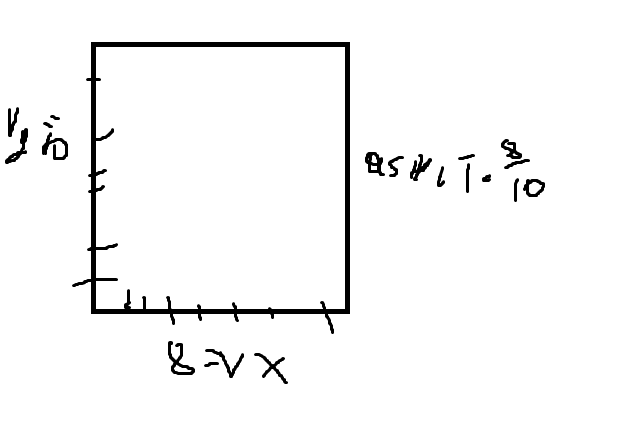
\includegraphics[width=0.50\linewidth]{1.png}
\end{figure}

\begin{figure} [H]
    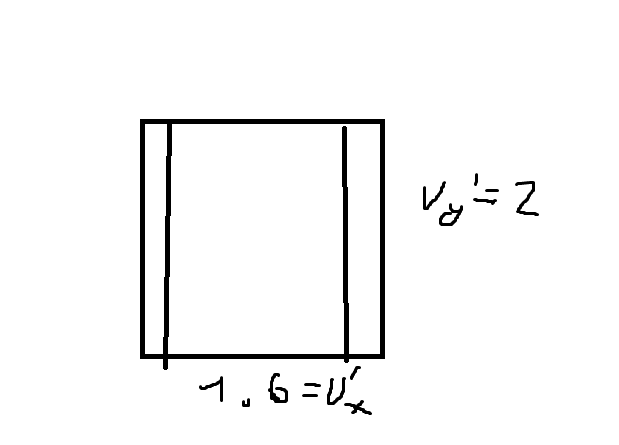
\includegraphics[width=0.50\linewidth]{2.png}
\end{figure}

\textbf{Команды:}

translate x  y


rotate $\vartheta$


scale S


figure 

Вспомогательные команды

popTransform - забираем из стка


pushTransform - добавляем в стек

\vspace{1cm}

scale 1.25

pushTransform

translate 0 -R

translate x y



translate -x -y

rotate 22.5

translate x y
\begin{figure} [H]
    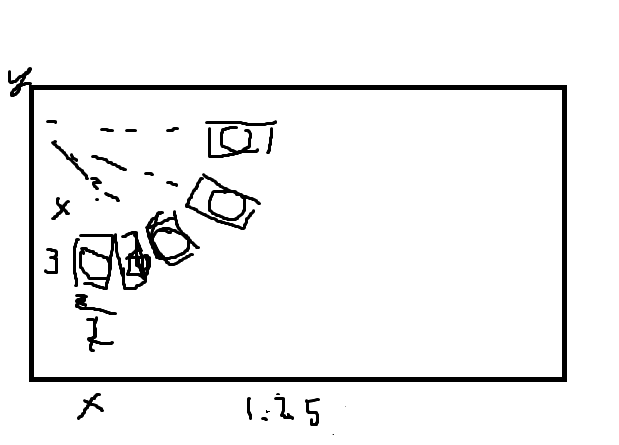
\includegraphics[width=0.50\linewidth]{3.png}
\end{figure}




Сокращение картинки:

scale 1.25

translate 0 -R

pushTransform

translate x y

figure

popTransform

rotate 22.5

pushTransform

translate x Y

figure


$\begin{cases}
    
pushTransform \\

rotate 22.5 \\

pushTransform \\

translate x y \\

figure \\

\end{cases}$

popTransform



\textbf{10.03.25}

\section{Операции над векторами}
\subsection{Двумерные вектора}
У веторов две характиристики:

длина

+

направлнение

Подобные вектора называется свободными векторами
если, есть точка из которой он начинается, 
то он называется связанным

Угол вектора $(r,\varphi)$

Угол ветора против часовой стрелки

\begin{figure} [H]
    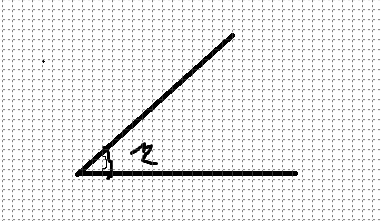
\includegraphics[width=0.50\linewidth]{Снимок экрана 2025-03-10 121857.png}
\end{figure}




\begin{figure} [H]
    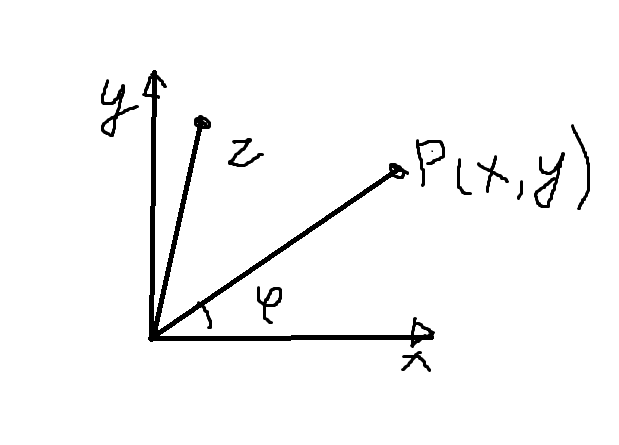
\includegraphics[width=0.50\linewidth]{4.png}
\end{figure}
Радиус вектор точка P

$\bar{P} (x,\varphi)$

$x = r cos \varphi$

$y = r sin \varphi$




\begin{figure} [H]
    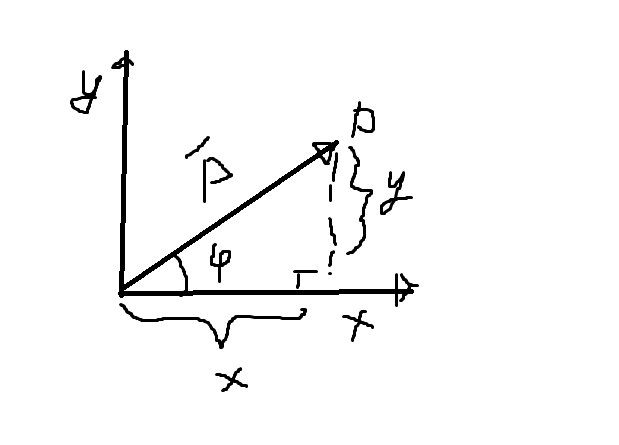
\includegraphics[width=0.50\linewidth]{5.png}
\end{figure}


\textbf{Сложение векторов(сумма)}

$\bar{u} u \bar{v}$

$\bar{u} + \bar{v}$


$\bar{u} = (u_x,u_y)$

$\bar{v} = (v_x,v_y)$

$\bar{u} + \bar{v} = (u_x+v_x,u_y+v_y)$


\begin{figure} [H]
    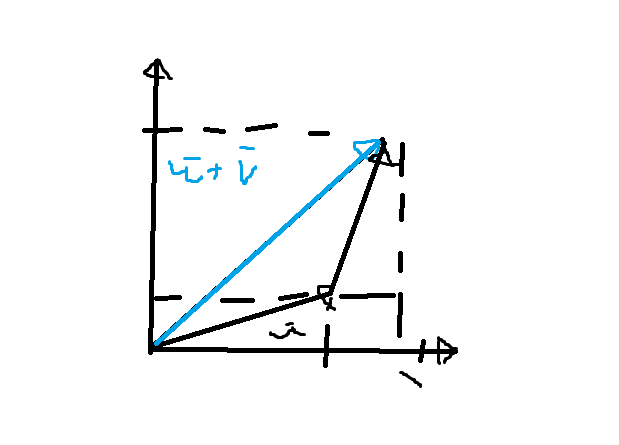
\includegraphics[width=0.50\linewidth]{6.png}
\end{figure}

\textbf{Разность векторов}
$\bar{u} u \bar{v}$

$\bar{u} - \bar{v}$


$\bar{u} - \bar{v} = (u_x-v_x,u_y-v_y)$

\begin{figure} [H]
    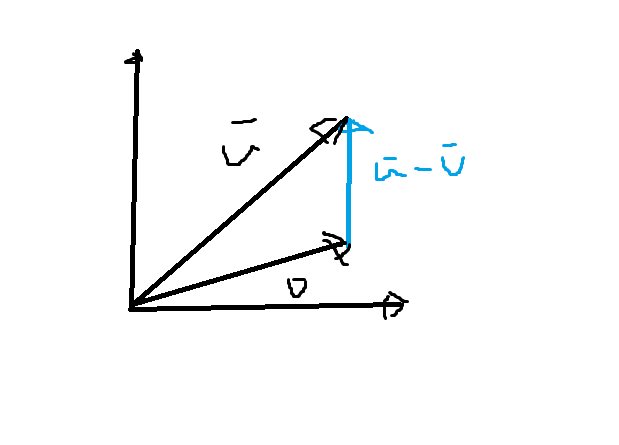
\includegraphics[width=0.50\linewidth]{7.png}
\end{figure}


\textbf{пупуп }


\begin{figure} [H]
    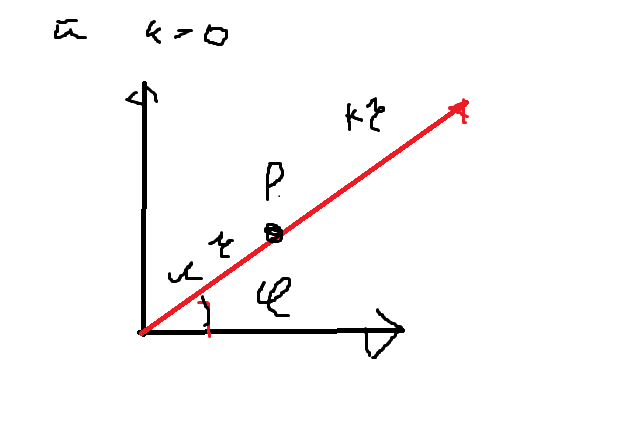
\includegraphics[width=0.50\linewidth]{8.png}
\end{figure}

$k\bar{u} = (ku_x,ku_y)$


\textbf{Скалярное произведение векторов}

$\bar{u}  \bar{v}$

$\bar{u} * \bar{v} = |\bar{u}| |\bar{v}| cos \widehat{\bar{u} \bar{v}} $

$\bar{u} = (r,\varphi)$

$|\bar{u}| = r$

$\bar{u} = \bar{u_x+\bar{u_y}}$

$\bar{u} * \bar{v} = (\bar{u_x+\bar{u_y}})*(\bar{v_x} + \bar{v_y})= $
$(|u_x|e_1 + |u_y|e_2) *(|v_x|e_1 *|v_x|e_1)$


$\bar{u}*\bar{v} = |\bar{u_x}||\bar{v_x}||\bar{u_x}+|\bar{v_y}| $ - основная формула
\begin{figure} [H]
    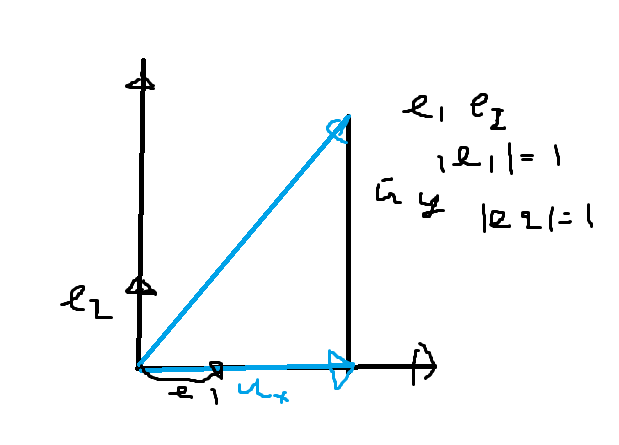
\includegraphics[width=0.50\linewidth]{9.png}
\end{figure}


$\bar{u} \bar{i}$

$\bar{u}*\bar{i} = |\bar{u}| |\bar{i}| cos \widehat{\bar{u} \bar{i}} =$
$|\bar{u}| cos\widehat{\bar{u} \bar{i}}$




\begin{figure} [H]
    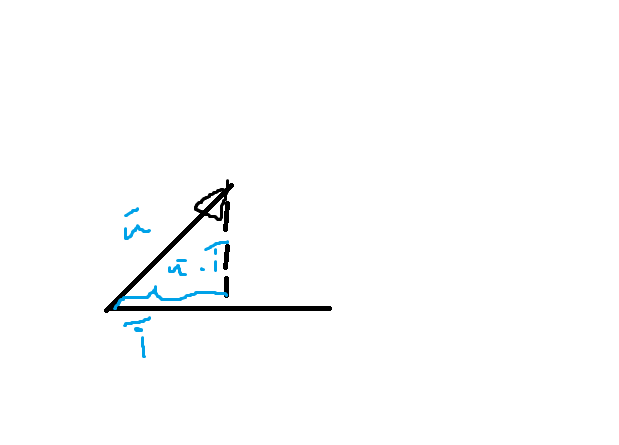
\includegraphics[width=0.50\linewidth]{10.png}
\end{figure}


dot-prodect - Скалярное произведение

\textbf{Псевдоскалярное произведение}

$\bar{u} \bar{v}$

$\bar{u} x \bar{v} = |\bar{u}|\bar{v}|sin < \bar{u} \bar{v}$

$\bar{u} x \bar{v} = -\bar{u} x \bar{v}$


$ e_1 x e_1 = 0
e_1 x e_2 = 1
e_2 x e_1 = -1
e_2 x e_2 = 0
= u_xv_y - u_yv_x > \bar{u} x \bar{v} = $ 
$ \begin{bmatrix}
    u_x & u_y \\
    v_x & v_y \\

\end{bmatrix} $

cross-prodect - Псевдоскалярное произведение 



\subsection{Трехмерные вектора}


\begin{figure} [H]
    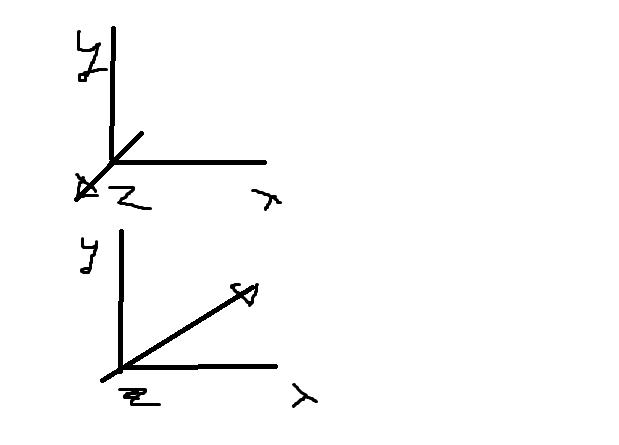
\includegraphics[width=0.50\linewidth]{КоординатыПравЛев.png}
    \text{Левосторонняя и правостороняя}
\end{figure}


\begin{figure} [H]
    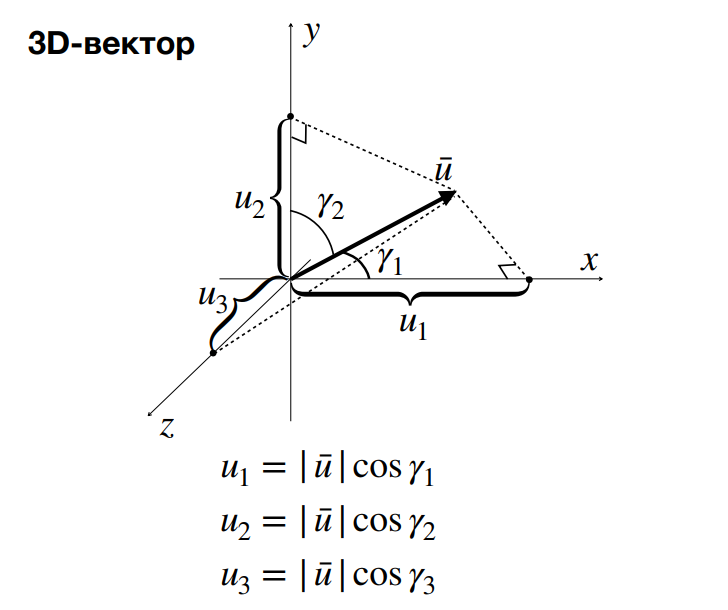
\includegraphics[width=0.50\linewidth]{Снимок экрана 2025-03-10 131058.png}
\end{figure}

\begin{figure} [H]
    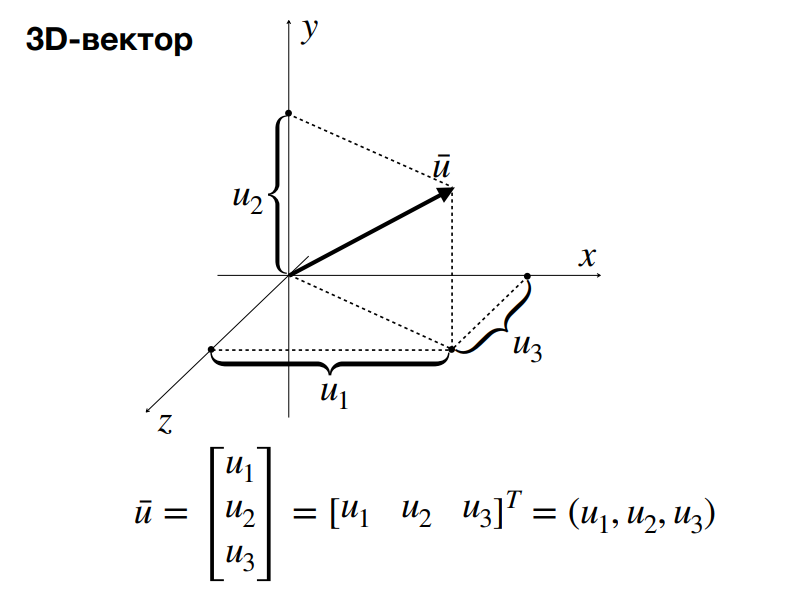
\includegraphics[width=0.50\linewidth]{Снимок экрана 2025-03-10 131148.png}
\end{figure}


\begin{figure} [H]
    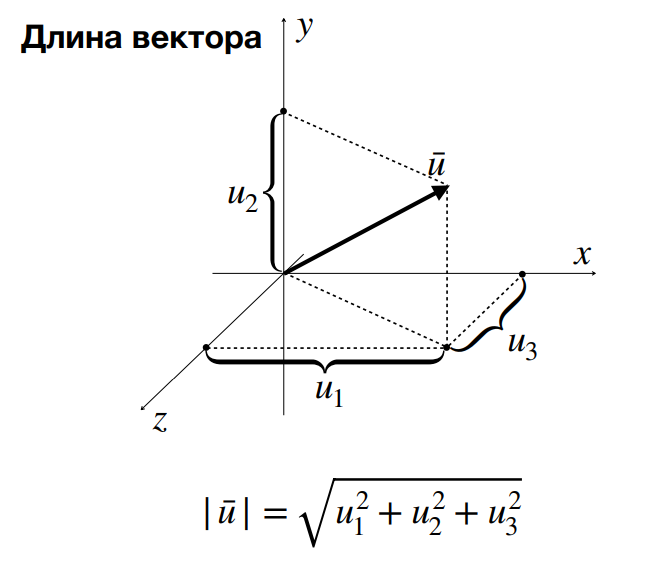
\includegraphics[width=0.50\linewidth]{Снимок экрана 2025-03-10 131219.png}
\end{figure}

\begin{figure} [H]
    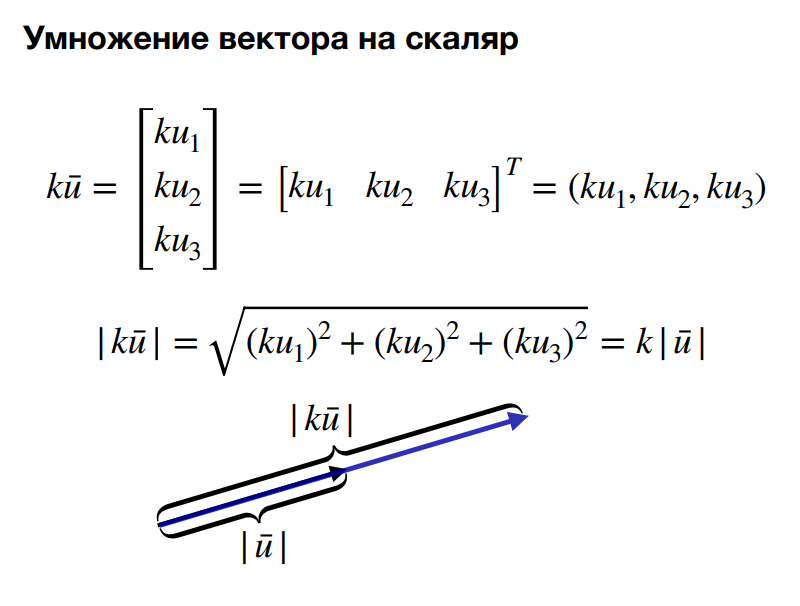
\includegraphics[width=0.50\linewidth]{Снимок экрана 2025-03-10 131255.png}
\end{figure}


\begin{figure} [H]
    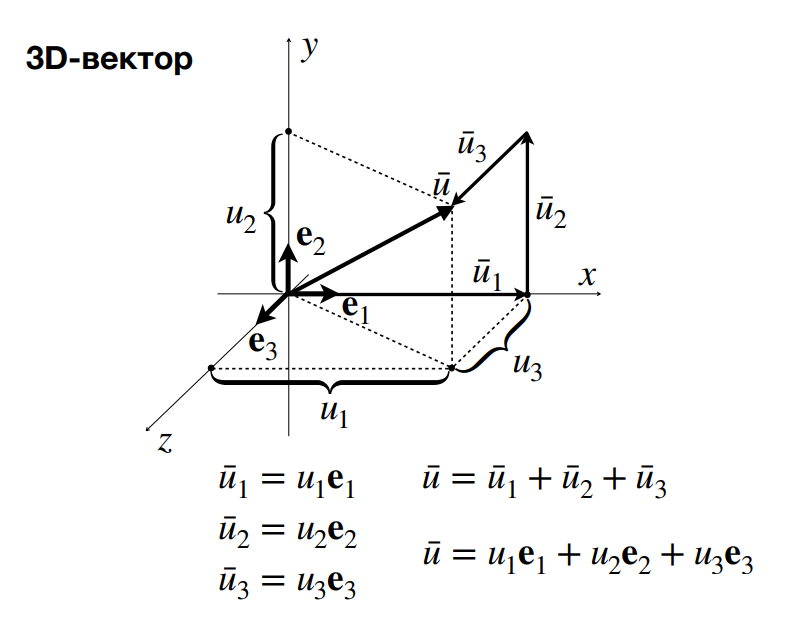
\includegraphics[width=0.50\linewidth]{Снимок экрана 2025-03-10 131408.png}
    \text{Сложение вектора по координатам}
\end{figure}


\textbf{!Скалярное произведение аналогично двухмерному}


\begin{figure} [H]
    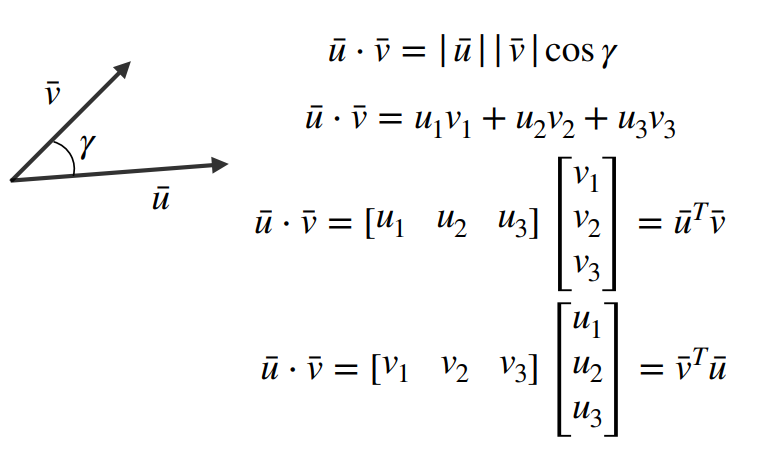
\includegraphics[width=0.50\linewidth]{Снимок экрана 2025-03-10 131719.png}
    \text{Через матрицу}
\end{figure}

\textbf{Векторное произведение}
\begin{figure} [H]
    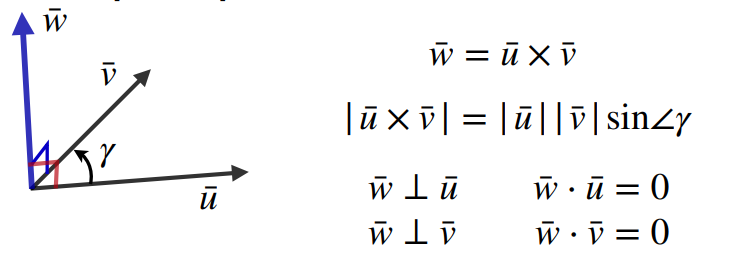
\includegraphics[width=0.50\linewidth]{Снимок экрана 2025-03-10 131820.png}
\end{figure}


Угол может быть как положительным, так и отрицательным

Не важно в какую сторону отмереяться угол

Если положительный результат, то вверх, 
отрицательный же вниз

\begin{figure} [H]
    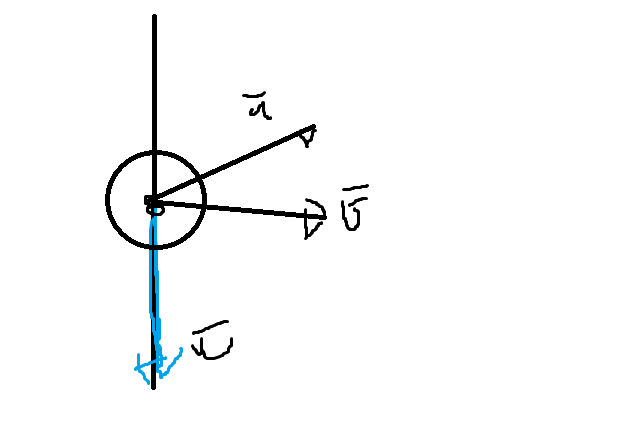
\includegraphics[width=0.50\linewidth]{11.png}
\end{figure}




\begin{figure} [H]
    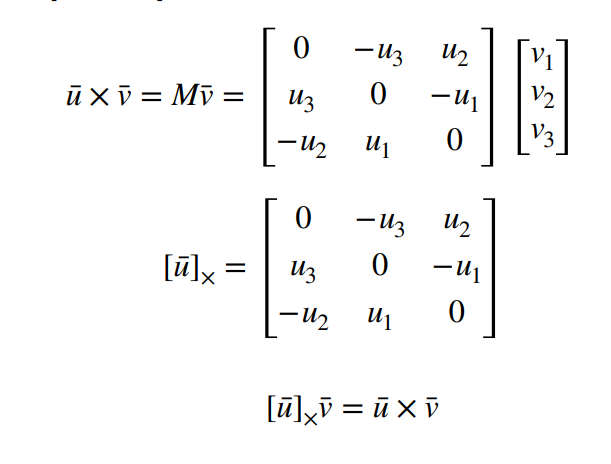
\includegraphics[width=0.50\linewidth]{Снимок экрана 2025-03-10 133749.png}
    \text{Матрица векторного произведения}
\end{figure}



\textbf{17.03.25}

\end{document}